\chapter{Ataque de Shamir al criptosistema de Merkle-Hellman} \label{ch:cuarto-capitulo}

    En este capítulo vamos a estudiar el método explicado por Shamir para romper el criptosistema recién explicado de Merkle-Hellman. En realidad, este ataque solo funciona para la ruptura del método básico, pero aun así, supuso el fin para este criptosistema. Nos adentraremos en la idea intuitiva para luego explicar el proceso de manera más formal. La fuente bibliográfica más importante es \cite{artSha}.
    
    \section{Introducción}

    El criptosistema de Merkle-Hellman era muy prometedor cuando apareció debido a su bajo coste computacional y su resistencia a la computación cuántica, por lo que era incluso preferido ante su principal competidor, RSA. Así fue hasta que Adi Shamir, en el año $1983$, rompió el criptosistema de Merkle-Hellman, dando fin a esta disyuntiva.

    Shamir comienza su artículo \cite{artSha} de la siguiente forma: ``El criptosistema Merkle-Hellman es uno de los dos principales criptosistemas de clave pública propuestos hasta ahora. Se demuestra que la variante básica de este criptosistema, en la que los elementos de la clave pública son múltiplos modulares de una secuencia supercreciente, se puede romper en tiempo polinómico''. A continuación, procedemos a explicar todo lo necesario para entender la idea que Shamir desarrolló en este documento.

    En primer lugar, debemos tener claro que la criptografía es una lucha interminable entre los creadores y los descifradores de código, y este trabajo no pretende dar ninguna respuesta definitiva en este sentido. Es más, el ataque criptoanalítico de Shamir sólo es efectivo para el criptosistema de una iteración propuesto por Merkle y Hellman, que es presumiblemente el menos seguro. Es decir, que este ataque no es aplicable a otros criptosistemas de clave pública propuestos en su artículo, como es el caso del método iterativo.

    Destacamos también alguna característica del algoritmo de Shamir, como es su eficiencia incluso en microcomputadores. No obstante, el propio Shamir explica que este algoritmo puede fallar en una clave concreta, aunque las heurísticas indican que estos fallos son extremadamente raros y que están respaldados por cientos de pruebas realizadas con claves de tamaño completo, en las que no se ha cometido ni un solo fallo.

    Recordemos primeramente que en el algoritmo básico de una iteración de Merkle-Hellman, lo que hacíamos era esconder la estructura de la sucesión supercreciente eligiendo dos valores, $M_{0}$ (el módulo) y $W_{0}$ (el multiplicador), tal que $M_{0} > \sum_{i=1}^{n} a'_{i}$, y que $W_{0}$ es primo relativo con $M_{0}$, es decir, gcd($M_{0}, W_{0}$) = $1$. Así, cada $a'_{i}$ se transforma en un nuevo valor entre $0$ y $M_{0} - 1$ según la multipliación modular siguiente:
    \begin{equation}
        a_{i} \equiv W_{0} \cdot a'_{i} \text{ mod } M_{0}
    \end{equation}
    La nueva sucesión $a = (a_{1}, ... , a_{n})$ se publica como la clave pública.
    
    Para demostrar que la complejidad asintótica del método criptoanalítico es polinómica, tenemos que considerar una familia de criptosistemas cuyo tamaño se incrementa indefinidamente. Hay dos parámetros básicos que tenemos que considerar: el número de elementos de la clave pública y su tamaño. Si estos se mantienen constantes, existe un algoritmo polinómico trivial para resolver los problemas de la mochila asociados. Por tanto, asumimos que el tamaño del módulo $M_{0}$ (y en consecuencia, también el tamaño de los elementos $a_{i}$) crece linealmente con $n$.

    Si denominados $d$ a la \textit{constante de proporcionalidad} ($1 < d < \infty$), debemos escoger el valor $a'_{1}$ con $dn - n$ bits, $a'_{i}$ con $dn - n + i - 1$ bits y $M_{0}$ con $dn$ bits de tamaño. El parámetro $d$ mide la redundancia introducida al criptosistema, es decir, la proporción entre los tamaños del texto cifrado y del texto plano. La complejidad de nuestro algoritmo es una función de $d$, que crece rápidamente, pero para cada valor fijo de $d$, es una función polinómica de $n$.

    \section{Descripción informal del algoritmo}

    El algoritmo propuesto por Shamir analiza los elementos de la clave pública $a = (a_{1}, ... , a_{n})$ y trata de encontrar una pareja de naturales $M$ y $W$ que funcionen como valores trampilla, tal que $W \cdot a_{i} \text{ mod } M$ sea una sucesión supercreciente y $M > \sum_{i=1}^{n} a_{i}$. Esto es, porque si se conoce cualquier par de números que cumplan con estas propiedades, entonces se pueden resolver eficientemente todos los problemas de la mochila relacionados con $a = (a_{1}, ... , a_{n})$ en tiempo lineal.

    Dado que los valores de $a$ se obtienen a partir de una secuencia supercreciente mediante multiplicación modular, sabemos que al menos existe una pareja, que es la escogida por el diseñador. Ciertamente, el algoritmo encuentra una pareja de valores trampilla, pero no garantiza que se encuentre ni el módulo original, ni el multiplicador que se utilizó en la construcción de la clave pública.

    Este algoritmo se divide en dos partes fundamentales. En la primera parte se utiliza el algoritmo de programación entera de Lenstra, para encontrar intervalos pequeños en $[0, 1]$ tal que siendo $M$ y $W$ una pareja de valores trampilla, entonces el ratio $W/M$ quede dentro de dicho intervalo.
    
    En la segunda parte del algoritmo, se usa el hecho de que conocemos el valor aproximado de $W/M$, para realizar un análisis más exhaustivo dividiendo cada intervalo en subintervalos más pequeños, de manera que si el ratio $W/M$ queda dentro de un subintervalo, entonces $M$ y $W$ componen una pareja de valores trampilla. Como ya hemos mencionado, al menos un subintervalo debe ser no vacío, ya que sabemos que existe una solución. Además, si utilizamos un algoritmo rápido de aproximación diofántica, encontraremos los valores más pequeños de $M$ y $W$ que verifican las condiciones.

    \begin{figure}[H]
        \centering
        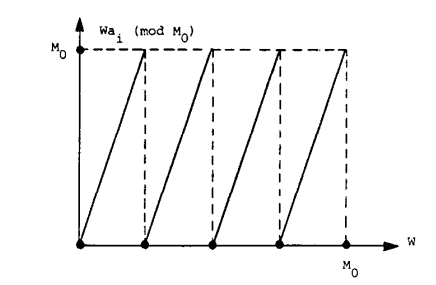
\includegraphics[width=0.6\textwidth, height=0.6\textheight, keepaspectratio]{Dientes_Shamir_1}
        \caption{Gráfica de la función $W \cdot a_{i} \text{ mod } M_{0}$, \cite{artSha}.}
        \label{fig:4.1}
    \end{figure}

    La figura \ref{fig:4.1} representa el gráfico de la función:
    \begin{equation}
        W \cdot a_{i} \text{ mod } M_{0} \text{ , con } 0 \leq W < M_{0}
    \end{equation}
    Esta imagen tiene forma de dientes de sierra. En ella, estamos representando $W$ en el eje horizontal y $M_{0}$ como el valor máximo del eje vertical, ya que es el módulo. La pendiente corresponde con el valor $a_{i}$, al igual que el número de mínimos; y la distancia entre dos mínimos sucesivos es igual a $M_{0}/a_{i}$, que es ligeramente superior a $1$.

    A continuación, vamos a resumir la idea principal para entender cómo se obtienen los valores $M_{0}$ y $W_{0}$. El valor $W_{0}$ verifica que $a'_{1} = W_{0} \cdot a_{1} \text{ mod } M_{0}$, es como máximo de tamaño $2^{dn - n}$. Como la pendiente es $a_{1}$, entonces la distancia horizontal entre $W_{0}$ y el mínimo más cercano de la curva $a_{1}$, no puede ser mayor a $2^{dn - n} / a_{1} \approx 2^{-n}$. Por tanto, la incógnita $W_{0}$ debe estar muy cerca de un mínimo de la curva $a_{1}$. Desafortunadamente, hay demasiados valores de $W_{0}$ y no podemos comprobar todos ellos.

    Sin embargo, podemos aplicar un análisis análogo a la curva $a_{2}$, por lo que $W_{0}$ también debe estar a una distancia de $2^{dn - n + 1} / a_{2} \approx 2^{-n + 1}$ del mínimo de $a_{2}$ más cercano. Consecutivamente, los mínimos de $a_{1}$ y $a_{2}$ deben estar muy cerca entre ellos. Esta condición de proximidad reduce el número de lugares en los que $W_{0}$ puede estar, aunque en la mayoría de casos sigue sin caracterizarlo de forma única.

    De igual manera, si superponemos más de estas funciones sierra en un gráfico, todas las posibles ubicaciones de $W_{0}$ deben estar cerca de un mínimo en cada curva. Así que, en lugar de encontrar un valor específico para $W_{0}$, debemos encontrar los puntos donde estos mínimos se agrupan, denominados \textit{puntos de acumulación}.

    Existe una sencilla regla empírica que podemos usar para tener una idea de cuántas de estas curvas debemos analizar al mismo tiempo, antes de que el conjunto de puntos de acumulación se reduzca a un tamaño manejable. Aunque esta estimación se ha probado en muchos experimentos y parece razonable, no siempre es totalmente precisa.

    Supongamos que $l$ representa la cantidad de curvas en forma de diente de sierra que superponemos en nuestro gráfico. Consideremos el $p$-ésimo mínimo de la curva $a_{1}$, que está situado en $W = pM_{0}/a_{1}$. Así, el mínimo más cercano de la curva $a_{i}$, se encuentra en algún lugar del intervalo:
    \begin{equation}
        [\frac{pM_{0}}{a_{1}} - \frac{M_{0}}{2a_{i}}, \frac{pM_{0}}{a_{1}} + \frac{M_{0}}{2a_{i}}]
    \end{equation}
    cuya longitud es de $\frac{M_{0}}{a_{i}} \approx 1$. A continuación, hacemos una suposición bastante razonable, aunque nada rigurosa, de que la localización real de los distintos mínimos de $a_{i}$ son variables aleatorias que siguen una distribución de probabilidad uniforme. Podemos así, estimar la probabilidad de que los mínimos de las curvas $a_{2}, ... , a_{l}$, estén lo suficientemente cerca del $p$-ésimo mínimo de la curva $a_{1}$, con la siguiente operación:
    \begin{equation}
        2^{-n + 1} \cdot 2^{-n + 2} \cdot \cdot \cdot 2^{-n + l - 1} \approx 2^{-ln + n + l^{2}/2}
    \end{equation}
    Puesto que debemos tener en cuenta también los $a_{1}$ posibles valores de $p$,
    \begin{equation}
        a_{1} \cdot 2^{(-ln + n + l^{2})/2} \approx 2^{dn - ln + n + l^{2}/2}
    \end{equation}
    Este valor es menor que $1$, cuando se verifica la siguiente desigualdad:
    \begin{equation}
        (l - d - 1)n > \frac{l^{2}}{2}
    \end{equation}
    Por último, tomando $n$ suficientemente grande, se verifica:
    \begin{equation}
        l > d + 1
    \end{equation}
    De esta manera, $l$ es una constante que depende de $d$, pero no de $n$. 
    
    La afirmación de que el número esperado de puntos de acumulación es menor que $1$ no es literal, ya que siempre hay al menos un punto de acumulación ``por construcción''. No obstante, es razonable suponer que en situaciones prácticas, cuando $l$ es mayor que $d + 1$, el punto ``construido'' no estará acompañado por otros puntos cercanos cuando se verifique la condición.

    \begin{ejemplo} \cite{artSha}
        Por ejemplo, tomando $n = 100$ y $|M| = 200$, $l = 4$ puede ser un candidato razonable para indicar el número de curvas en forma de diente de sierra.
    \end{ejemplo}

    Sin embargo, todavía tenemos dos problemas: cómo deshacerse de $M_{0}$, cuyo valor aún es desconocido; y cómo encontrar los puntos de acumulación de los mínimos de las $l$ curvas. Un punto a tener en cuenta es que los puntos de acumulación dependen de las pendientes de las curvas, pero no de su tamaño. Por tanto, si dividimos entre $M_{0}$ los dos ejes en la curva $i$-ésima, obtenemos la curva de la siguiente función:
    \begin{equation}
        V \cdot a_{i} \text{ mod } 1 \text{ , con } 0 \leq V < 1
    \end{equation}
    Siendo $V = W/M_{0}$. Además, esta curva es independiente de $M_{0}$, como se aprecia en la imagen:

    \begin{figure}[H]
        \centering
        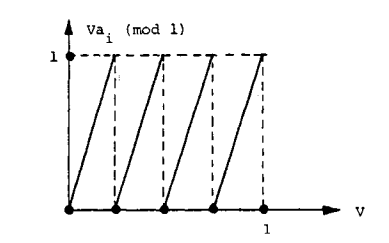
\includegraphics[width=0.6\textwidth, height=0.6\textheight, keepaspectratio]{Dientes_Shamir_2}
        \caption{Gráfica de la función $V \cdot a_{i} \text{ mod } 1$, \cite{artSha}.}
    \end{figure}

    En el nuevo sistemas de coordenadas, la pendiente de la curva sigue siendo $a_{i}$, al igual que el número de mínimos; pero la distancia entre mínimos sucesivos se reduce a $1/a_{i}$. Así, el parámetro $W_{0}$ queda reemplazado por el parámetro $V_{0} = W_{0}/M_{0}$, y la distancia entre este parámetro y el mínimo de la curva $a_{i}$ más cercano, se reduce aproximadamente en $2^{dn}$. El problema de localización de los puntos de acumulación de $l$ mínimos en el nuevo sistema de coordenadas, puede describirse mediante desigualdades lineales con $l$ incógnitas integrales. Las condiciones para que el $p$-ésimo mínimo de $a_{1}$, $q$-ésimo mínimo de $a_{2}$, $r$-ésimo mínimo de $a_{3}$, ..., estén suficientemente próximos entre sí, son las siguientes:
    \begin{align}
        \text{Sean } p,q,r, ... , \text{ enteros, } &&1 \leq p \leq a_{1} - 1 \\
        -\epsilon_{2} \leq \frac{p}{a_{1}}-\frac{q}{a_{2}} \leq \epsilon'_{2} &&1 \leq q \leq a_{2} - 1 \\
        -\epsilon_{3} \leq \frac{p}{a_{1}}-\frac{r}{a_{3}} \leq \epsilon'_{3} &&1 \leq r \leq a_{3} - 1
    \end{align}
    \hspace{5cm}\vdots\hspace{5cm}\vdots
    
    donde $\epsilon_{i}$ y $\epsilon'_{i}$ representan las desviaciones hacia a la derecha y hacia la izquierda de $p/a_{1}$. multiplicando las inecuaciones dobles de la columna izquierda por sus denominadores, obtenemos:
    \begin{align}
        -\delta_{2} \leq pa_{2} &- qa_{1} \leq \delta'_{2} \\
        -\delta_{3} \leq pa_{3} &- ra_{1} \leq \delta'_{3} \\
        &\vdots
    \end{align}
    Aquí se muestra que los valores de $a_{2}, a_{3}, ... ,$ se reducen simultáneamente a valores absolutos pequeños cuando se multiplica por $p$ y se reduce mod $a_{1}$.

    El problema de minimizar simultáneamente dos números mediante multiplicación modulo un tercer número, puede resolverse utilizando un sencillo algoritmo de fracciones continuas. En el caso general, debemos utilizar el algoritmo de programación entera de Lenstra, que aunque es más lento, es polinomial respecto al tamaño de los coeficientes para un número fijo de incógnitas. Este algoritmo es esencialmente un procedimiento de decisión que nos dice si un cierto sistema de desigualdades lineales tiene soluciones enteras. Al utilizar búsqueda binaria en los bits sucesivos de $p$, podemos encontrar todos los puntos de acumulación de las $l$ curvas.

    \begin{figure}[H]
        \centering
        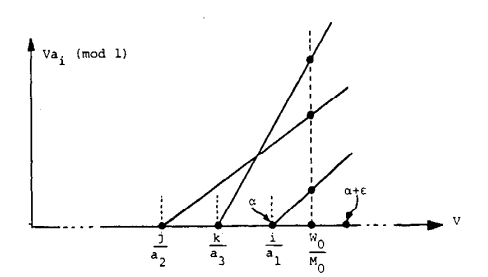
\includegraphics[width=0.6\textwidth, height=0.6\textheight, keepaspectratio]{Dientes_Shamir_3}
        \caption{Sección ampliada del diagrama superpuesto cerca de $V_{0} = \frac{W_{0}}{M_{0}}$, \cite{artSha}.}
    \end{figure}

    Para controlar el tiempo de ejecución del algoritmo y que sea polinomial, debemos añadir un parámetro $k$, el cual se encarga de abortar el programa si se supera cierto número $k$ de puntos de acumulación (tomaremos $k = 100$ por defecto). Un ejemplo extremo de no utilizar este parámetro, sería que todos los $a_{i}$ fueran iguales, por lo que todos los mínimos serían puntos de acumulación. Otra idea que podemos usar es cambiar el valor de $l$ y de $k$, ya que así es posible controlar la fracción de claves para las que el algoritmo no consigue calcular una pareja de valores trampilla.
    
    \begin{observacion}
        Cabe mencionar que no resolver todas las instancias de un problema no es una desventaja grave en el contexto de la criptografía, ya que un criptosistema se vuelve inútil cuando la mayoría de sus claves pueden ser criptoanalizados eficientemente, por lo que no hace falta que se resuelvan todas.
    \end{observacion}

    Podría suceder que un usuario, futuro receptor de un mensaje, permutase los elementos de su clave pública antes de mostrarla. Entonces, $a_{i}$ ya no correspondería al $i$-ésimo elemento más pequeño de la sucesión supercreciente. Aún así, esta variante de Merkle-Hellman puede romperse en tiempo polinómico con esta técnica. Como sólo debemos buscar los $l$ elementos más pequeños, estos se pueden encontrar en $O(n')$ maneras. Dado que $l$ es una constante que no depende de la complejidad de $n$, nuestro método aumenta su complejidad en un factor polinomial. 

    Alternativamente, el criptoanalista puede relajar los valores de $\epsilon$, que representan las desviaciones entre los distintos mínimos de la curva, de modo que el problema de programación entera pueda satisfacerse no sólo cuando se adivinen correctamente los $l$ valores incrementales más pequeños, sino para cualquier elección de $l$ valores lo suficientemente pequeños. Además, si se eligen adecuadamente los nuevos valores de los $\epsilon$, es posible sustituir el factor $O(n')$ por una constante, lo que en aplicaciones prácticas ahorra tiempo.

    El análisis de las primeras $l$ curvas en diente de sierra, nos permite concentrarnos en unas pocas regiones pequeñas en las que debe localizarse el valor real de $V_{0} = W_{0}/M_{0}$. Dentro de estas regiones, las curvas son lineales a trozos con sólo unos pocos puntos de discontinuidad, por lo que sus valores pueden expresarse y compararse sin un análisis excesivo de casos.

    La segunda parte del algoritmo se encarga de descartar en estas regiones, todas aquellas subregiones en las que la sucesión de valores de la curva no sea supercreciente, o su suma sea menor que $1$. Cada punto racional del resto de subregiones corresponde a una pareja de valores trampilla. Además como $V_{0} = W_{0}/M_{0}$ no ha sido descartado, algún subconjunto es no vacío.

    Sea ahora $p$ uno de los valores obtenido por la primera parte del algoritmo. Consideramos el intervalo $[p/a_{1}, (p+1)/a_{1})$ entre $a_{1}$ mínimos sucesivos. El número de puntos de discontinuidad esperados de otras curvas superpuestas en él, es $O(n)$. Sea $V_{1}, ... , V_{s}$ una lista de coordenadas de estos puntos discontinuos ordenadas de manera creciente. Entre cada $V_{t}$ y $V_{t+1}$, todas las curvas $a_{i}$ parecen segmentos lineales simples. El $i$-ésimo segmento lineal puede expresarse así:
    \begin{equation}
        Va_{i} - \tau^{t}_{i} \text{ , con } V_{t} \leq V < V_{t+1}
    \end{equation}
    donde $\tau^{t}_{i}$ es el número de mínimos de $a_{i}$ en $(0, V_{t}]$. Esto es, $\tau^{t}_{i}/a_{i}$ es el punto donde se corta la línea con el eje $V$. A continuación, podemos escribir el rango, tamaño y las condiciones de sucesión supercreciente de la siguiente forma:
    \begin{align}
        &V_{t} \leq V < V_{t+1} \\
        \sum_{i=1}^{n} &(Va_{i} - \tau^{t}_{i}) < 1 \\
        Va_{i} - \tau^{t}_{i} > &\sum_{j=1}^{i-1} (Va_{j} - \tau^{t}_{j}) \text{ , con } i = 2, ... , n
    \end{align}
    La solución de este sistema de inecuaciones lineales en $V$ es un subintervalo de la forma $[V_{t}, V_{t+1})$, posiblemente vacío. Además, se verifica que $W/M$ pertenece a ese subintervalo para algún $p$ y $t$, si y solo si, $M$ y $W$ forman una pareja de valores trampilla.

    Solo falta mencionar que, en caso de que se realice una permutación de elementos de la sucesión supercreciente, es necesario usar también la condición de permutación supercreciente. Como no se puede averiguar la permutación aplicada en tiempo polinomial, debemos usar que toda sucesión supercreciente es una sucesión creciente, para reducir el número de permutaciones posibles a considerar. 

    Para ello, debemos ampliar la definición de la secuencia $V_{1}, ... , V_{s}$, incluyendo no solo los puntos de acumulación, sino también las $V$ coordenadas de las intersecciones entre pares de curvas. Esto puede hacer que aumente el valor de $s$, pasando de $O(n)$ a $O(n^2)$. 
    
    Dentro de cada nuevo rango de valores $[V_{t}, V_{t+1})$, existe una forma clara de ordenar las diferentes curvas verticalmente. Por lo tanto, solo hay una forma posible de organizar sus nombres de manera que la secuencia sea creciente. En particular, de las $n!$ permutaciones posibles, sólo debemos considerar $O(n^2)$ en cada punto de acumulación.
    
    \section{Descripción formal del algoritmo}

    Como ya mencionamos anteriormente, el algoritmo abortará si las $l$ curvas tienen al menos $k$ puntos de acumulación. En esta sección vamos a analizar cómo la fracción de los parámetros $l$ y $k$, influye en la cantidad de fallos del algoritmo y demostraremos que en un modelo probabilístico simplificado, esta fracción pueden hacerse arbitrariamente pequeña.
    
    Por simplificar, asumimos que $a_{1}$ es un valor primo fijo y que $a_{2}, ... , a_{l}$ son variables aleatorias independientes que siguen una distribución de probabilidad uniforme en $[1, a_{1} - 1]$. La condición de que $a_{1}$ sea primo es básicamente para que los inversos modulares estén bien definidos, pero no es esencial y por tanto, se puede reemplazar por otra condición o un análisis más cuidadoso. Por último, asumiremos por simplicidad que las variables del algoritmo de programación entera $\delta_{i}$ y $\delta'_{i}$ coinciden, y denotaremos ambas variables como $\delta$, aunque esto sea un abuso de notación. 

    \begin{definicion} \cite{artSha}
    Para cada $2 \leq i \leq l$, se define $S_{i}$ como el conjunto de indices de mínimos de $a_{1}$ suficientemente cercanos a algún mínimo de $a_{i}$:
        \begin{equation}
            S_{i} = \{1 \leq p \leq a_{1} - 1 \text{ | }\exists \text{ } q_{i} \text{, } 1 \leq q_{i} \leq a_{i} - 1, \text{ tq } -\delta \leq pa_{i} - qa_{1} \leq \delta\}    
        \end{equation}
    \end{definicion}

    Como todos los $S_{i}$ son conjuntos de mínimos de $a_{1}$, su intersección $S_{2} \cap ... \cap S_{l}$, es exactamente el conjunto de puntos de acumulación en los que un mínimo de $a_{1}$, está simultáneamente cerca de los mínimos de todas las demás curvas.

    \begin{lema} \cite{artSha}
        Mostramos ahora una caracterización alternativa al conjunto $S_{i}$ definido previamente, más fácil de manipular:
        \begin{equation}
            S_{i} = \{j_{i}a_{i}^{-1} \text{ mod } a_{1} \text{ | } -\delta \leq j_{i} \leq \delta \text{, } j_{i} \neq 0\}    
        \end{equation}
    \end{lema}

    \begin{proof}
        \begin{equation}
            p \equiv j_{i}a_{i}^{-1} \text{ mod } a_{1}
        \end{equation}
        equivale a
        \begin{equation}
            pa_{i} \equiv j_{i}a_{i}^{-1}a_{i} \text{ mod } a_{1} \equiv j_{i} \text{ mod } a_{1}
        \end{equation}
        y por tanto, existe $q_{i}$ tal que:
        \begin{equation}
            pa_{i} = j_{i} + q_{i}a_{1}
        \end{equation}
        Como $-\delta \leq j_{i} \leq \delta$, $pa_{i}-q_{i}a_{1}$ cumple las condiciones. Finalmente, el valor $j_{i} = 0$ no está permitido en la definición de $S_{i}$, por lo que se restringe ese valor.
    \end{proof}

    La equivalencia $p \equiv j_{i}a_{i}^{-1} \text{ mod } a_{1}$, establece para cada $p$, una relación uno a uno entre la secuencia $a_{2}, ... , a_{l}$ y la secuencia $j_{2}, ... , j_{l}$. El valor $p$ es un punto de acumulación de $a_{2}, ... , a_{l}$, sí y solo si todos los correspondientes $j_{i}$ son enteros no nulos pertenecientes a $[-\delta, \delta]$. De manera alternativa, cuando $p$ y una secuencia de $j_{i}$ son dados, existe una única secuencia de $a_{i}$ para la cual $p$ es un punto de acumulación con estos $j_{i}$ índices.

    \begin{lema} \cite{artSha} \label{lem:4.5}
        Sean $p'$ y $p''$ dos puntos de acumulación de $a_{2}, ... , a_{l}$, y sean $j'_{2}, ... , j'_{l}$ y $j''_{2}, ... , j''_{l}$ las secuencias de sus índices $j$ asociados. Si $\delta < \sqrt{a_{1}/2}$, entonces ambas secuencias son múltiplos de una secuencia común $j_{2}, ... , j_{l}$ donde se verifica que gcd($j_{2}, ... , j_{l}$) = $1$.
    \end{lema}

    \begin{proof}
        Partiendo de $p' \equiv j'_{i}a_{i}^{-1} \text{ mod } a_{1}$, y $p'' \equiv j''_{i}a_{i}^{-1} \text{ mod } a_{1}$, podemos obtener:
        \begin{equation}
            a_{i} \equiv j'_{i}p'^{-1} \equiv j''_{i}p''^{-1} \text{ mod } a_{1}
        \end{equation}
        que, tras simplificación:
        \begin{equation}
            j'_{i}j_{i}^{''-1} \equiv p'p^{''-1} \text{ mod } a_{1}
        \end{equation}
        Como la parte derecha de la equivalencia no depende de $i$, para cualquier $s$ y $t$ se verifica:
        \begin{align}
            j'_{s}j_{s}^{''-1} &\equiv j'_{t}j_{t}^{''-1} \text{ mod } a_{1} \\
            j'_{s}j''_{t} &\equiv j'_{t}j''_{s} \text{ mod } a_{1}
        \end{align}
        Por la suposición de $\delta$, cada producto $j'j"$ sólo puede estar en $[\frac{-a_{1}}{2}, \frac{a_{1}}{2}]$, por lo que se cumple (incluso sin módulo):
        \begin{equation}
            j'_{s}j''_{t} = j'_{t}j''_{s}
        \end{equation}
        Esta igualdad se verifica para todo $s$ y $t$ sólo si las secuencias $j'$ y $j"$ son múltiplos racionales entre sí. Como contienen sólo números enteros, deben ser múltiplos de alguna secuencia común $j_{2}, ... , j_{l}$ de enteros, cuyo gcd sea $1$.
    \end{proof}

    \begin{corolario}
        Cuando $\delta < \sqrt{a_{1}/2}$ y la intersección $S_{2} \cap ... \cap S_{l}$ es no vacía, hay un punto de acumulación cuya secuencia de índices es $j_{2}, ... , j_{l}$ y su gcd es $1$, y además todos los puntos de acumulación restantes se obtienen multiplicando la secuencia de $j_{i}$ por $1, -1, 2, -2, 3, -3, ...$ etc. hasta que un elemento supere el valor de $\delta$.

        Cuando $\delta \geq \sqrt{a_{1}/2}$, la intersección $S_{2} \cap ... \cap S_{l}$ es más complicada de analizar y no tenemos ninguna caracterización sencilla.
    \end{corolario}

    \begin{definicion} \cite{artSha}
        Denotaremos como $N(l, k, \delta)$ al número de secuencias $a_{2}, ... , a_{l}$ en $[1, a_{1} - 1]$, para las que la intersección $S_{2} \cap ... \cap S_{l}$ contiene al menos $k$ puntos cuando la distancia tolerable es $\delta$.
    \end{definicion}

    Nos interesa la probabilidad condicional de que las $l$ curvas tengan al menos $k$ puntos de acumulación, cuando se sabe que tienen al menos uno. Dado que lo primero implica lo segundo, esta probabilidad condicional es simplemente:
    \begin{equation}
        \frac{N(l, k, \delta)}{N(l, 1, \delta)} 
    \end{equation}

    \begin{lema} \cite{artSha}
        Para cada $\delta < \sqrt{a_{1}/2}$ y $l \geq 3$, hay una constante $\tau$ en $[3/\pi^{2}, 1/2]$ que depende solo de $l$, tal que:
        \begin{equation}
            N(l, 1, \delta) \approx \tau(a_{1} - 1)(2\delta)^{l - 1}
        \end{equation}
    \end{lema}
    
    \begin{proof}
        Podemos calcular el número de secuencias $a_{2}, ... , a_{l}$ que tienen al menos un punto de acumulación, contando el número de secuencias $p, a_{2}, ... , a_{l}$, donde $p$ es un punto de acumulación de $a_{i}$. Este número es igual al número de secuencias $p, j_{2}, ... , j_{l}$, donde $p$ es arbitrario y los $j_{i}$ son enteros no nulos pertenecientes a $[-\delta, \delta]$, equivalentamente, $(a_{1} - 1)(2\delta)^{l - 1}$. Para corregir el cálculo, tomamos solamente secuencias de $j_{i}$ cuyo gcd sea $1$. Por el lema \ref{lem:4.5}, para cada $a_{i}$, hay exactamente dos secuencias $j_{i}$ con puntos de acumulación y con gcd = $1$ (cada secuencia es la negación de la otra). 
        
        Para $l = 3$, la fracción de secuencias enteras de longitud $l - 1$ cuyo gcd = $1$, converge a $6/\pi^{2}$ y para valores superiores de $l$ esta fracción se aproxima a $1$. Dado que cada secuencia $a_{i}$ con puntos de acumulación se cuenta exactamente dos veces, tenemos que dividir esta constante por $2$ para obtener la constante correcta $\tau$.
    \end{proof}

    \begin{lema} \cite{artSha}
        Si $\delta < \sqrt{a_{1}/2}$, entonces $N(l, k, \delta) \leq N(l, 1, \frac{\delta}{k/2})$.
    \end{lema}
    
    \begin{proof}
        Sea $j_{2}, ... , j_{l}$ la secuencia de índices con gcd = $1$, cuya existencia está garantizada por el lema \ref{lem:4.5}. Como $a_{2}, ... , a_{l}$ tiene al menos $k$ puntos de acumulación, esta secuencia de $j_{i}$ puede ser multiplicada por $k/2$ y todos sus elementos seguirán perteneciendo a $[-\delta, \delta]$. Como consecuencia, todos los $j_{i}$ originales están en $[\frac{-\delta}{k/2}, \frac{\delta}{k/2}]$, y por tanto, la sucesión $a_{i}$ tiene al menos un punto de acumulación incluso cuando el límite $\delta$ se sustituye por otro límite más estricto $\frac{\delta}{k/2}$.
    \end{proof}

    Llegamos a continuación al teorema principal de este capítulo.

    \begin{teorema} \cite{artSha} \label{theo:4.10}
        Cuando $\delta < \sqrt{a_{1}/2}$ y $l \geq 3$, el valor de la probabilidad condicionada $\frac{N(l, k, \delta)}{N(l, 1, \delta)}$ es como máximo $(\frac{1}{k/2})^{l - 1}$. 
    \end{teorema}

    \begin{proof}
        \begin{align}
           \frac{N(l, k, \delta)}{N(l, 1, \delta)} &\leq \frac{N(l, 1, \delta/(k/2))}{N(l, 1, \delta)} \\
            &= \frac{\tau(a_{1} - 1)(2\delta/(k/2))^{l - 1}}{\tau(a_{1} - 1)(2\delta)^{l - 1}} \\
            &= (\frac{1}{k/2})^{l - 1}
        \end{align}
    \end{proof}

    \begin{ejemplo} \cite{artSha}
        Tomando $l = 4$, $k = 100$ y $\delta < \sqrt{a_{1}/2}$, la probabilidad de que $4$ curvas de dientes en sierra tengan al menos $100$ puntos de acumulación cuando se sabe que tienen al menos uno, es de $(1/50)^{3} = 1/125000$. Por tanto, si utilizamos el algoritmo de Lenstra (algoritmo L$^{3}$) para encontrar los puntos de acumulación y se aborta tras encontrar $100$ puntos, la probabilidad de fallo es insignificante.
    \end{ejemplo}

    En nuestro análisis aplicado, $\delta$ es aproximadamente $2^{dn - n}$ y $a_{1}$ es aproximadamente $2^{dn}$. Así, la condición $\delta < \sqrt{a_{1}/2}$ es equivalente a la condición $d < 2$. Shamir no pudo probar el limite superior del Teorema \ref{theo:4.10} para criptosistemas en los que la relación $d$, del tamaño del módulo entre el número de elementos, es mayor que $2$. Sin embargo, Jeff Lagarias anunció posteriormente un límite superior diferente aplicable a todo el rango $1 < d < \infty$.

    \section{Análisis del algoritmo}

    En el apartado anterior se ha mostrado que todos los criptosistemas de una iteración de Merkle-Hellman pueden ser rotos en tiempo polinomial con probabilidad de fallo arbitrariamente pequeña. La parte que más tiempo necesita es la aplicación del algoritmo de programación entera de Lenstra, ya que en el peor caso su complejidad es polinomial en $n$, pero exponencial en $l$.

    Una característica muy importante del ataque propuesto, es que se dirige a la clave pública y no a los textos cifrados individuales. De este modo, el criptoanalista puede abordar claves de reserva o de bajo volumen, incluso antes de que se utilicen por primera vez. Además, podría dedicar meses de tiempo computacional a cada clave, con el fin de facilitar posteriormente la decodificación del mensaje en microsegundos.

    El problema más importante que queda abierto en este capítulo, es la seguridad criptográfica sobre los criptosistemas de Merkle-Hellman de varias iteraciones. En cada iteración, el módulo elegido aleatoriamente debe ser mayor que la suma de los elementos, por lo que las multiplicaciones modulares inversas reducen simultáneamente el tamaño de los elementos al menos en $log(n)$. En principio, esta condición permite hallar el único intervalo en el que se encuentra $W/M$, pero no $W$ ni $M$. 

    En el caso de la mochila de iteración simple, cualquier pareja trampilla era útil, ya que generaba una secuencia supercreciente fácilmente resoluble. En el caso de las mochilas de iteración múltiple, sólo los valores $W$ y $M$ correctos permiten al criptoanalista hacer la multiplicación inversa correctamente y atacar las iteraciones internas una a una.

\endinput